\documentclass[mathserif]{beamer}

\usepackage{listings}
\usepackage{showexpl}
\usepackage{setspace}
\usepackage{multirow}
\usepackage{dtklogos}
\usepackage{caption}
\usepackage{subcaption}
\usepackage[T1]{fontenc}

%\usepackage{handoutwithnotes}

%\pgfpagesuselayout{3 on 1 with notes}[a4paper,border shrink=5mm]

%\pgfpageslogicalpageoptions{1}{border code=\pgfusepath{stroke}}
%\pgfpageslogicalpageoptions{2}{border code=\pgfusepath{stroke}}
%\pgfpageslogicalpageoptions{3}{border code=\pgfusepath{stroke}}

\lstdefinestyle{latexsty}{
	language={[LaTeX]TeX},
    basicstyle=\small\ttfamily,
    breaklines=true,
    breakindent=0pt, 
    backgroundcolor=\color{lightgray},
    numbers=none, numberstyle=\tiny, stepnumber=1, numbersep=5pt,
    commentstyle=\color{red},
    showstringspaces=false,
    keywordstyle=\color{blue}\bfseries,
    morekeywords={align,begin},
    tabsize=2,
    pos=b
}

\usetheme{default}
\useoutertheme{infolines}
\usecolortheme[RGB={166,5,20}]{structure}
%\setbeamertemplate{items}[circle]
\setbeamertemplate{blocks}[rounded][shadow=false]
\setbeamertemplate{navigation symbols}{}
\setbeamertemplate{caption}[numbered]


\title{\LaTeX: An Introduction (Part 2)}
\subtitle{University Graduate College Training Course}
\author[Martin Chorley]{Dr Martin Chorley}
\institute[COMSC]{School of Computer Science \& Informatics, Cardiff University}
\date[21/02/14]{February 21st, 2014}


\begin{document}

%--------------- slide -------------------
\begin{frame}[plain]
	\titlepage
\end{frame}
	

%--------------- slide -------------------
\begin{frame}{Introduction}

\vfill
\begin{itemize}
	\item Recap of Beginners \LaTeX
	\item Floating Environments
	\item Cross Referencing
	\item \BibTeX
	\item Defining Custom Environments
	\item Defining Custom Commands
	\item Presentations
		\begin{itemize}
			\item Beamer class
			\item Creating slides
		\end{itemize}	
\end{itemize}
\vfill
\end{frame}


%--------------- slide -------------------
\begin{frame}{Schedule}
\vfill
	\begin{description}
		\item[\textbf{09:00 - 09:15}] Welcome \& Introduction
		\item[\textbf{09:15 - 10:30}] Basic \LaTeX, Exercise 1, Floats, \texttt{figure} environment, Exercise 2
		\item[\textbf{10:30 - 11:00}] \textbf{Coffee Break}
		\item[\textbf{11:00 - 12:30}] Referencing with \BibTeX, Exercise 3
		\item[\textbf{12:30 - 13:30}] \textbf{Lunch}
		\item[\textbf{13:30 - 15:00}] Presentations in \LaTeX - \texttt{beamer}
		\item[\textbf{15:00 - 15:30}] \textbf{Coffee Break}
		\item[\textbf{15:30 - 17:00}] Preamble, Custom Environments \& Commands, Exercises, \LaTeX\ helpdesk
		\item[\textbf{17:00}] Close
	\end{description}
\vfill
\end{frame}

%--------------- slide -------------------
\begin{frame}{\LaTeX\ Recap}


\vfill
Hopefully, everyone is happy with these \LaTeX\ concepts:
\vfill
\begin{itemize}
	\item Writing \LaTeX\ files
	\item Document Classes \& Structure
	\item Packages
	\item Sections \& Chapters
	\item Text Formatting
	\item Tables
	\item Lists
	\item Typesetting Maths
\end{itemize}
\vfill

\end{frame}



%--------------- slide -------------------
\begin{frame}{Recap - Writing \LaTeX\ Files}

Creating documents with~\LaTeX\ is simple:
\vfill
\begin{enumerate}
	\item Write our document as plain text in a `\texttt{.tex}' file, using~\LaTeX\ commands to structure and format it 	\item Compile our `\texttt{.tex}' file to produce the output
\end{enumerate}
\vfill
\end{frame}



%--------------- slide -------------------
\begin{frame}[fragile]
\frametitle{Recap - First (basic)~\LaTeX\ Example}
	\begin{LTXexample}[style=latexsty]
		\documentclass{article}
		    % Preamble goes here
		    \begin{document}
		        % Document content goes here
		        Hello World!
		    \end{document}
	\end{LTXexample}
	
\end{frame}
	


%--------------- slide -------------------
\begin{frame}[fragile]
\frametitle{Recap - Writing \LaTeX\ -- Commands}

\LaTeX\ commands have an effect on the text in the document. Some commands have additional arguments or optional parameters. The general syntax for a~\LaTeX\ command is:

\vfill
		\texttt{{\textbackslash}commandname[opt1, opt2, \ldots]\{arg1\}\{arg2\}\ldots}

\vfill

\end{frame}

%--------------- slide -------------------
\begin{frame}[fragile]
\frametitle{Recap - Writing \LaTeX\ -- Commands \& Whitespace}

Whitespace after~\LaTeX\ commands will generally be ignored. If you need a space after a command, you can either add an empty parameter to the command, or use a (breaking or non-breaking) space command.
\vfill
	\begin{LTXexample}[style=latexsty]
		\LaTeX commands will ignore whitespace after them.\newline
		We can force a space after a \LaTeX{} command using an empty parameter. \\
		Or we can use a space command (texttt{\ } or \texttt{~} )after our \LaTeX\ command.
		This way our \LaTeX~commands and text do not flow together!
	\end{LTXexample}
\vfill

\end{frame}


%--------------- slide -------------------
\begin{frame}[fragile]
\frametitle{Recap - Writing \LaTeX\ -- Comments}

The `\texttt{\%}' character is used to create comments in~\LaTeX. When~\LaTeX\ is processing your \texttt{.tex} file and it comes across a `\texttt{\%}', it ignores the rest of the line.

	\begin{LTXexample}[style=latexsty]
		%This is a comment and will not be shown.
		Here is some text in our file that will be shown. %but the rest of the line will not be.
		We can even do things like br%
		eak words up with comm%
		ents if we want to.
	\end{LTXexample}

\end{frame}


%--------------- slide -------------------
\begin{frame}
\frametitle{Recap - Compiling}

That's more than you need to create a basic \texttt{.tex} file and create your first document.

\vfill
To compile your \texttt{.tex} file and create your document, you use a~\LaTeX\ compiler:

\vfill
\begin{itemize}
	\item \texttt{latex} calls the \texttt{tex} compiler and outputs \texttt{.dvi} files
	\item \texttt{pdflatex} calls the \texttt{pdftex} compiler and outputs \texttt{.pdf} files
\end{itemize}
\vfill
\end{frame}


%--------------- slide -------------------
\begin{frame}
\frametitle{Recap - Compiling}
\vfill
Compiling creates a lot of extra files, including the output of your document. All of these files are recoverable and can be remade by re-compiling, so can be deleted safely.

\vfill
The only files you always need to keep and should not delete are \texttt{.tex}, \texttt{.cls}, \texttt{.sty}, \texttt{.bib} and \texttt{.bst}.
\vfill

\end{frame}


%--------------- slide -------------------
\begin{frame}[fragile]
\frametitle{Recap - Document Structure}

Every~\LaTeX\ document must have a certain structure:
\vfill
\begin{lstlisting}[style=latexsty]
\documentclass{...}
% Preamble here
\usepackage{...}
\begin{document}
    % Document contents here
    ...
\end{document}
\end{lstlisting}
\vfill
The area before \texttt{{\textbackslash}begin\{document\}} is called the \emph{preamble}. It contains commands concerning the setup of the document. 
\vfill
The text of your document is enclosed between the \texttt{{\textbackslash}begin\{document\}} and \texttt{{\textbackslash}end\{document\}}, within the `document' \emph{environment}.
\end{frame}


%--------------- slide -------------------
\begin{frame}[fragile]
\frametitle{Recap - Environments}

Environments enclose text and cause it to be treated a certain way, similar to commands. They usually have a larger scope than a command though. They begin with \texttt{{\textbackslash}begin\{\ldots\}} and end with \texttt{{\textbackslash}end\{\ldots\}}

	\begin{LTXexample}[style=latexsty]
		\begin{document}
		    Here is some text
		    \begin{center}
		    	    Here is some centred text
		    \end{center}
		\end{document}
	\end{LTXexample}

\end{frame}

%--------------- slide -------------------
\begin{frame}[fragile]
\frametitle{Recap - Document Class}

The \texttt{{\textbackslash{documentclass\{\ldots\}}}} command tells~\LaTeX\ which type of document we are creating, and how it should be set up and formatted. This command usually comes at the very beginning of the file. 
\vfill
As with many commands it has optional parameters, which will change aspects of the structure, formatting or layout.
\vfill
\begin{lstlisting}[style=latexsty]
\documentclass[opt1,opt2,...]{class}
\end{lstlisting}
\vfill

\end{frame}

%--------------- slide -------------------
\begin{frame}
\frametitle{Recap - Document Class}

\LaTeX\ comes with many types of document class built in. Some of the most commonly used are:
\vfill
\begin{center}
\begin{tabular}{r | l}
\texttt{article} & for scientific articles, short reports, papers etc. \\
\texttt{IEEEtran} & for articles in the IEEE Transactions format. \\
\texttt{report} & for longer reports containing chapters, small books, theses. \\
\texttt{books} & for real books \\
\texttt{beamer} & for writing presentations \\
\end{tabular}
\end{center}
\end{frame}

%--------------- slide -------------------
\begin{frame}[fragile]
\frametitle{Recap - Document Class Example}

So, to make a two-sided \texttt{article} in 12pt font on A4 paper, you can use the command:
\vfill
\begin{lstlisting}[style=latexsty]
\documentclass[12pt,a4paper,twoside]{article}
\end{lstlisting}
\vfill

\end{frame}


%--------------- slide -------------------
\begin{frame}[fragile]
\frametitle{Recap - Top Matter}

After we've specified the document class and included any packages we want to use, we can define information about the document in the top matter. 
\vfill
\begin{lstlisting}[style=latexsty]
\documentclass{article}

\title{Document Title}
\author{Me}
\date{February 2013}

\begin{document}
    \maketitle
\end{document}
\end{lstlisting}
\vfill

\end{frame}

%--------------- slide -------------------
\begin{frame}[fragile]
\frametitle{Recap - Abstract}

Usually, scientific papers and reports will have an abstract, so \LaTeX\ includes an environment for specifying which part of your document is the abstract. \texttt{article} and \texttt{report} document classes can use the \texttt{abstract} environment.
\vfill
\begin{lstlisting}[style=latexsty]
\documentclass{article}

\begin{document}
    \begin{abstract}
        ...
        Abstract goes here
        ...    
    \end{abstract}
    \ldots
\end{document}
\end{lstlisting}
\vfill

\end{frame}

%--------------- slide -------------------
\begin{frame}
\frametitle{Recap - Sections \& Chapters}

We often want to break documents into different parts, chapters or sections. 
\vfill
\begin{center}
	\begin{tabular}{l | c }
		Command & Level \\
		\hline
		\texttt{{\textbackslash}part\{part\_title\}} & -1  \\
		\texttt{{\textbackslash}chapter\{chapter\_title\}} & 0 \\
		\texttt{{\textbackslash}section\{section\_title\}} & 1 \\
		\texttt{{\textbackslash}subsection\{subsection\_title\}} & 2 \\
		\texttt{{\textbackslash}subsubsection\{subsubsection\_title\}} & 3 \\
		\texttt{{\textbackslash}paragraph\{paragraph\_title\}} & 4 \\
		\texttt{{\textbackslash}subparagraph\{subparagraph\_title\}} & 5 \\		
	\end{tabular}
\end{center}
\vfill
Which section commands you can use depends on which document class you are using. 

\end{frame}

%--------------- slide -------------------
\begin{frame}[fragile]
\frametitle{Recap - Packages}

Often,the default set of commands available to~\LaTeX\ cannot solve all of our problems alone. To include graphics, use coloured text or other complicated functionality you will need to include extra packages. 
\vfill
These packages will often have extra optional parameters:
\begin{lstlisting}[style=latexsty]
\usepackage[opt1, opt2, ...]{packagename}
\end{lstlisting}
\vfill

So, for example, to use the package allowing us to use coloured text:
\begin{lstlisting}[style=latexsty]
\usepackage{color}
\end{lstlisting}
\vfill

\end{frame}

%--------------- slide -------------------
\begin{frame}[fragile]
\frametitle{Recap - Packages}

We can include multiple packages in the \texttt{{\textbackslash}usepackage} command:
\begin{lstlisting}[style=latexsty]
\usepackage{color,graphicx,geometry}
\end{lstlisting}
\vfill

Any packages where we want to set optional parameters need to use their own~\texttt{{\textbackslash}usepackage} command:
\begin{lstlisting}[style=latexsty]
\usepackage{color,graphicx}
\usepackage[margin=2cm]{geometry}
\end{lstlisting}
\vfill

\end{frame}

%--------------- slide -------------------
\begin{frame}[fragile]
\frametitle{Basic LaTeX Example - Exercise 1}
\vfill
So, we can put all this together, and create a simple \LaTeX\ document.
\vfill
\end{frame}


%--------------- slide -------------------
\begin{frame}
\frametitle{Floats}
\vfill
When using a WYSIWYG editor (such as Word), it is common to control \emph{exactly} where pictures or tables are placed in the text. However, many scientific publications allow pictures or tables to go on separate dedicated pages, or at other points in the document in order to not disrupt the flow of the text. \LaTeX\ handles this using \emph{floating environments}. 
\vfill
It can be disconcerting to `let go' of the control of where items are placed in your document at first, but in general it results in better looking and easier to read documents.
\vfill
\end{frame}

%--------------- slide -------------------
\begin{frame}[fragile]
\frametitle{Floating Tables}
\vfill
In order to make a table `floating' we wrap the \texttt{tabular} environment in a \texttt{table} environment. This makes the table float so that \LaTeX\ can place it in the most appropriate location within the document. It also allows us to add a caption and label to our table.
\vfill
	\begin{LTXexample}[style=latexsty]
		\begin{table}[ position specifier ]
			\centering
			\begin{tabular}{|l|}
				... your table here ...
			\end{tabular}
			\caption{This is my table}
			\label{tab:mytable}
		\end{table}
	\end{LTXexample}
\vfill
\end{frame}

%--------------- slide -------------------
\begin{frame}[fragile]
\frametitle{Position Specifier}
\vfill
The optional position specifier on a floating environment gives a `hint' to \LaTeX\ as to where you want to place the table. \LaTeX\ will try and honour this position, but it is not guaranteed. The options for location specifier are:
\vfill
\begin{center}
	\begin{tabular}{r | l}
		Position \\ Specifier & Location \\
		\hline
		\texttt{h} & \textbf{h}ere - where the table is declared \\
		\texttt{t} & at the \textbf{t}op of the page \\
		\texttt{b} & at the \textbf{b}ottom of the page \\
		\texttt{p} & on a special \textbf{p}age of floats \\
	\end{tabular}
\end{center}
\vfill
Note that \texttt{h} is automatically replaced by \texttt{ht}, as it can cause problems when used alone. You can try and force \LaTeX\ to use a specific position by adding \texttt{!} to the specifier.
\vfill
\end{frame}


%--------------- slide -------------------
\begin{frame}[fragile]
\frametitle{Cross Referencing}
\vfill
If our tables (and later images) are `floating' around the document, they may end up being in a different location to the text describing them. \LaTeX\ provides methods for cross-referencing within documents.
\vfill
\texttt{{\textbackslash}label} allows us to label floats and sections:
\vfill
\begin{lstlisting}[style=latexsty]
	\label{label_name}
\end{lstlisting}
\vfill
\texttt{{\textbackslash}ref} allows us to refer back to the labelled float or section:
\vfill
\begin{lstlisting}[style=latexsty]
	\ref{label_name}
\end{lstlisting}
\vfill
\texttt{{\textbackslash}page ref} allows us to refer to the page the labelled float or section is on:
\vfill
\begin{lstlisting}[style=latexsty]
	\pageref{label_name}
\end{lstlisting}
\vfill
When using any form of referencing we are required to compile our document twice, so that \LaTeX\ is able to work out where our references should point to within the document.
\vfill
\end{frame}

%--------------- slide -------------------
\begin{frame}[fragile]
\frametitle{Cross Referencing}
\vfill
\begin{lstlisting}[style=latexsty]
		\begin{table}[htb]
		    \centering
		    \begin{tabular}{|l|}
		        ... your table here ...
		    \end{tabular}
		    \caption{This is my table}
		    \label{tab:mytable}
		\end{table}
		Now in my text I can refer to the Table~\ref{tab:mytable}.
	\end{lstlisting}
\vfill
\end{frame}


%--------------- slide -------------------
\begin{frame}[fragile]
\frametitle{\texttt{Figure} environment}
\vfill
The \texttt{figure} environment allows us to `float' our images, much like the \texttt{table} environment allows us to `float' our \texttt{tabular} environments.
\vfill
As a floating environment, it is then possible to label and caption our images.
\vfill
\begin{lstlisting}[style=latexsty]
	\begin{figure}[placement option]
	    ... figure contents ....
	\end{figure}
\end{lstlisting}
\vfill
\end{frame}

%--------------- slide -------------------
\begin{frame}[fragile]
\frametitle{\texttt{Figure} environment}
\vfill
	\begin{LTXexample}[style=latexsty]
	\begin{figure}[ht!]
		\centering
	    
\includegraphics[width=0.4\textwidth]{img/background}
	    \caption{I have no idea what this is}	    
	\end{figure}
	\end{LTXexample}
\vfill
\end{frame}


%--------------- slide -------------------
\begin{frame}[fragile]
\frametitle{Subfigures}
\vfill
It is often desired to combine multiple images or figures within a single floating environment. For this we can use the \texttt{subcaption} package.
\vfill
\begin{lstlisting}[style=latexsty]
	\usepackage{graphicx}
	\usepackage{subcaption}
	\begin{figure}[htbp]
	    \centering
	    \begin{subfigure}{0.3\textwidth}
	        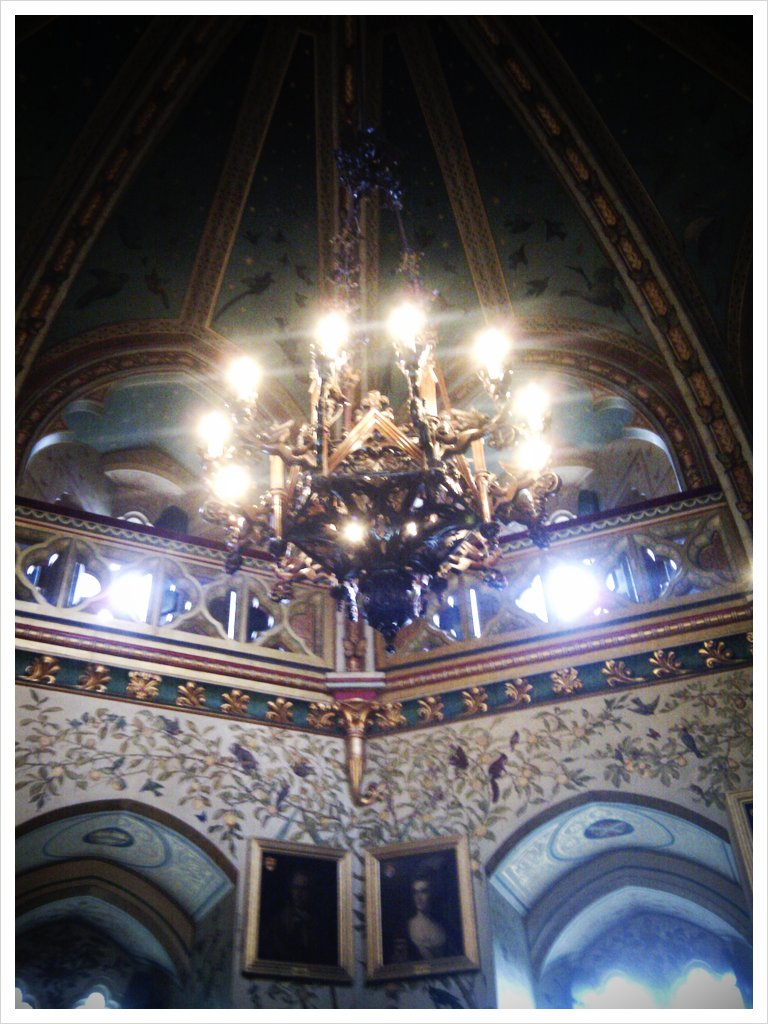
\includegraphics[width=\textwidth]{img/lights}
	        \caption{Some lights}
	    \end{subfigure}
	    \begin{subfigure}{0.3\textwidth}
	        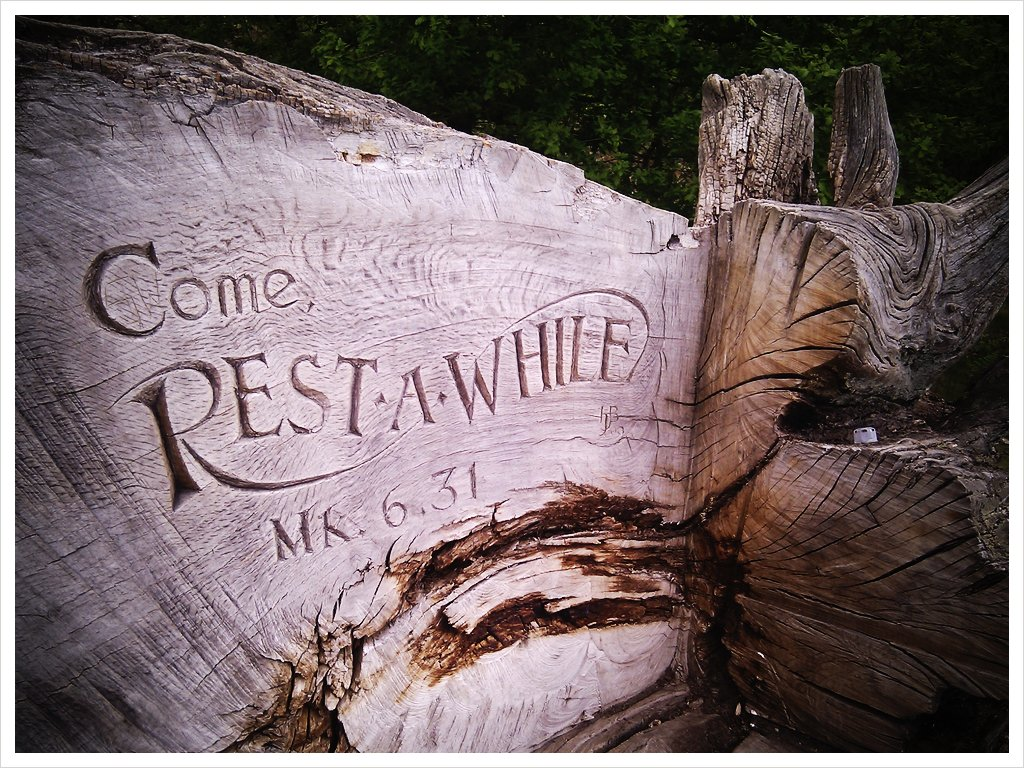
\includegraphics[width=\textwidth]{img/bench}
	        \caption{A bench}
	    \end{subfigure}
	    \caption{Some lights and a bench}
	\end{figure}
\end{lstlisting}
\vfill
\end{frame}

%--------------- slide -------------------
\begin{frame}[fragile]
\frametitle{Subfigures}
	\begin{figure}[htbp]
	    \centering
	    \begin{subfigure}{0.3\textwidth}
	        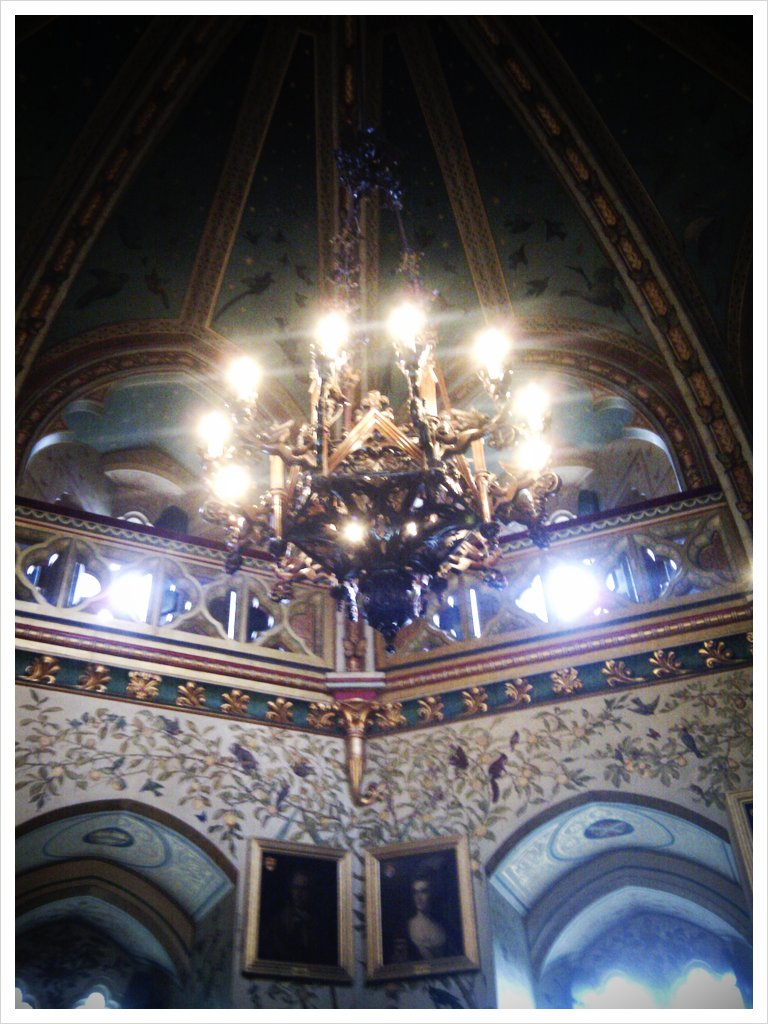
\includegraphics[width=\textwidth]{img/lights}
	        \caption{Some lights}
	    \end{subfigure}
	    \begin{subfigure}{0.3\textwidth}
	        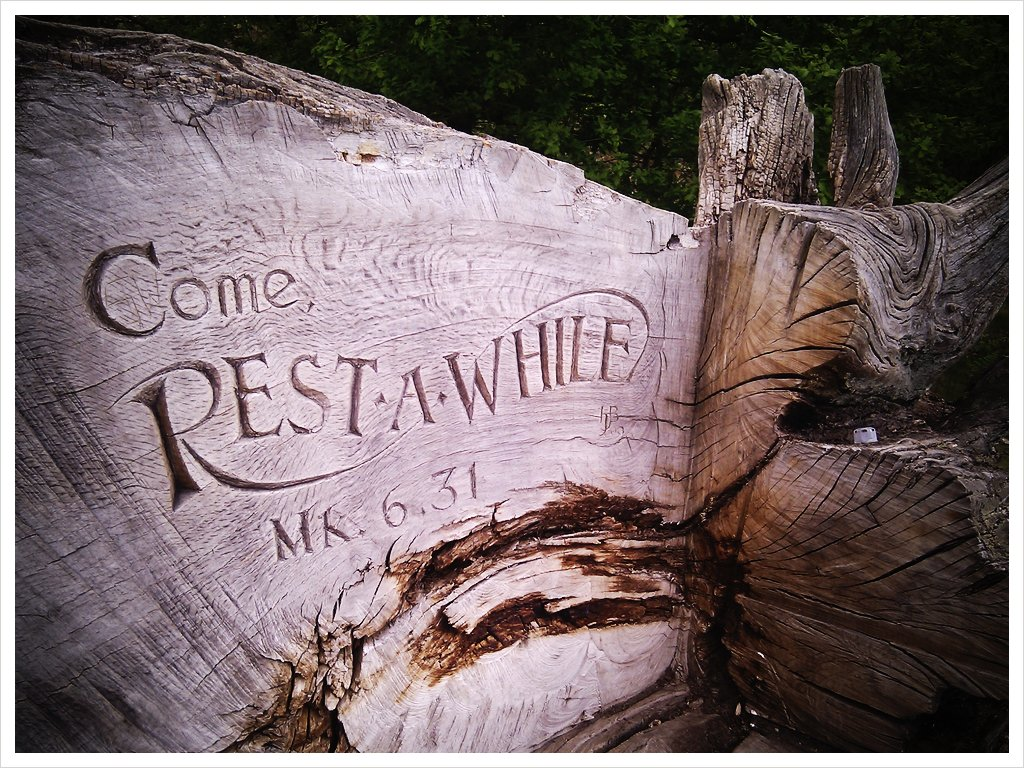
\includegraphics[width=\textwidth]{img/bench}
	        \caption{A bench}
	    \end{subfigure}
	    \caption{Some lights and a bench}
	\end{figure}
\end{frame}


%--------------- slide -------------------
\begin{frame}[fragile]
\frametitle{Subfigures - alignment}
\vfill
We can supply position options to the \texttt{subfigure} environment to align the images within a subfigure
\vfill
\begin{lstlisting}[style=latexsty]
	\usepackage{graphicx}
	\usepackage{subcaption}
	\begin{figure}[htbp]
	    \centering
	    \begin{subfigure}[b]{0.3\textwidth}
	        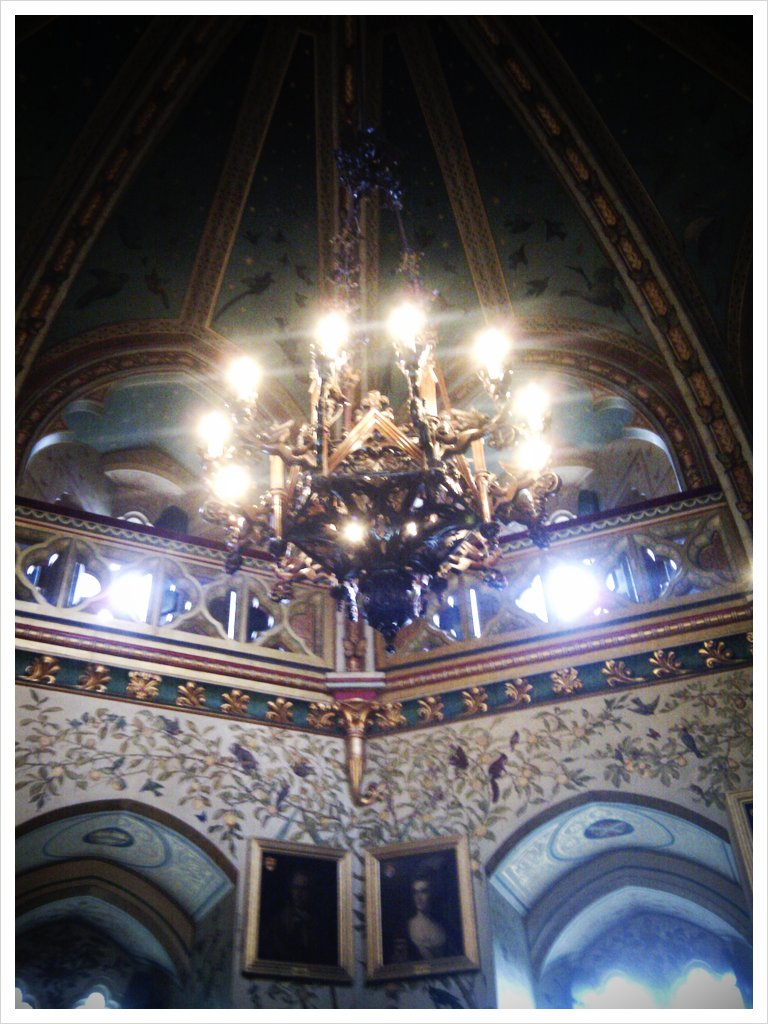
\includegraphics[width=\textwidth]{img/lights}
	        \caption{Some lights}
	    \end{subfigure}
	    \begin{subfigure}[b]{0.3\textwidth}
	        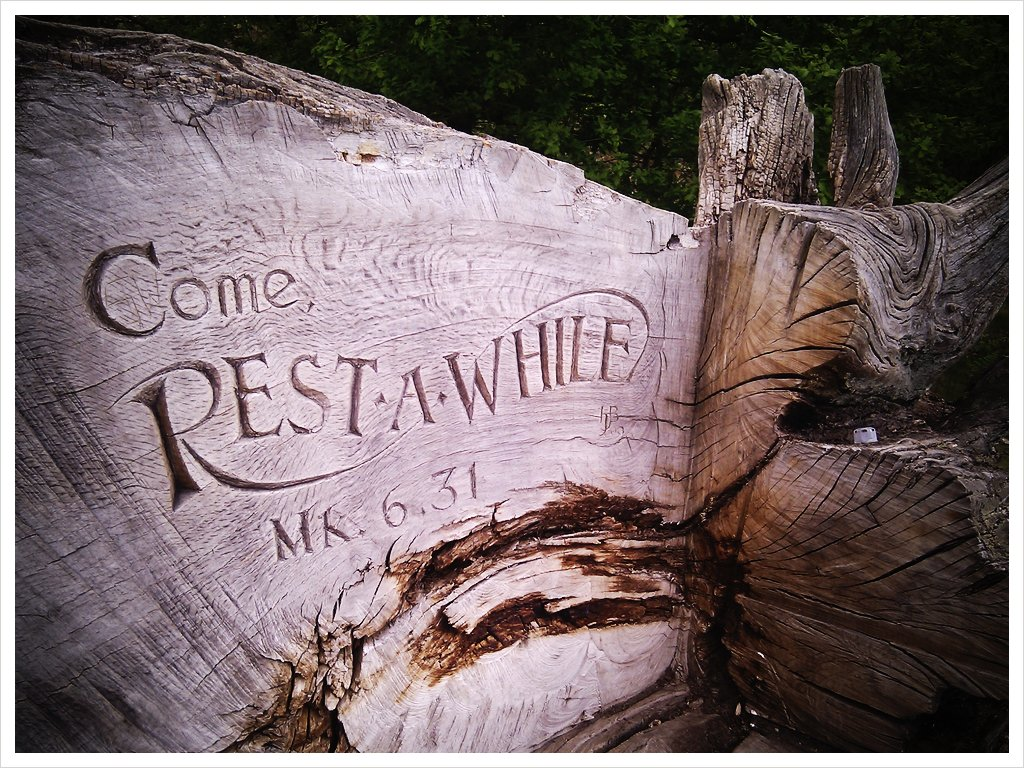
\includegraphics[width=\textwidth]{img/bench}
	        \caption{A bench}
	    \end{subfigure}
	    \caption{Some lights and a bench}
	\end{figure}
\end{lstlisting}
\vfill
\end{frame}

%--------------- slide -------------------
\begin{frame}[fragile]
\frametitle{Subfigures}
	\begin{figure}[htbp]
	    \centering
	    \begin{subfigure}[b]{0.3\textwidth}
	        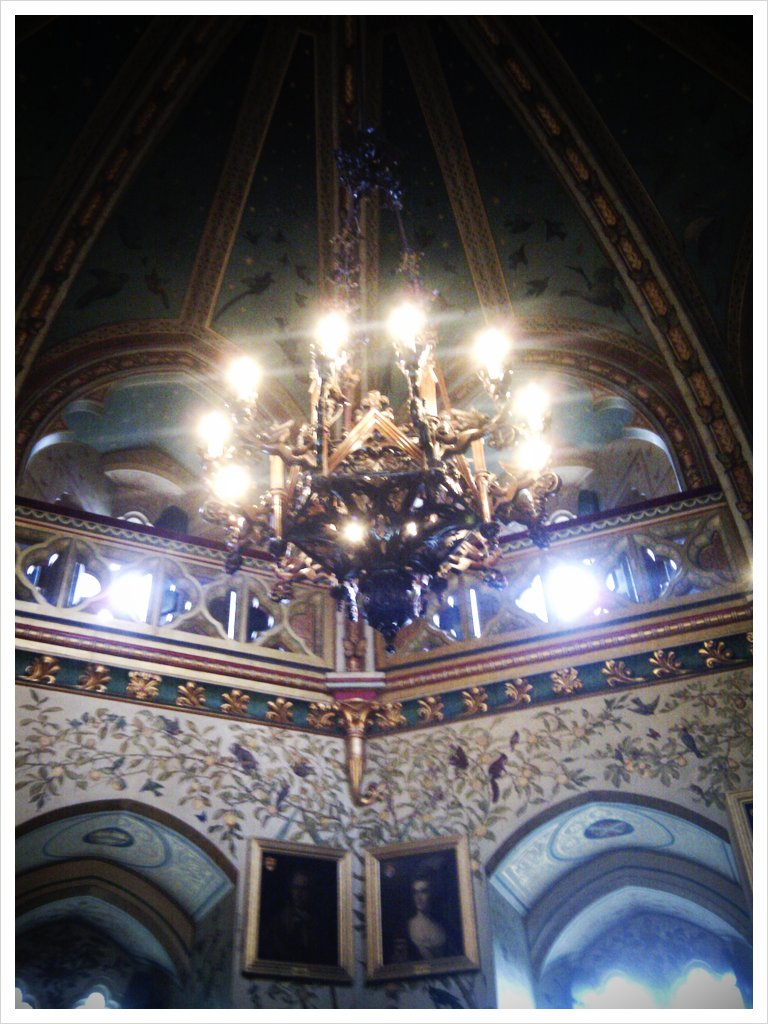
\includegraphics[width=\textwidth]{img/lights}
	        \caption{Some lights}
	    \end{subfigure}
	    \begin{subfigure}[b]{0.3\textwidth}
	        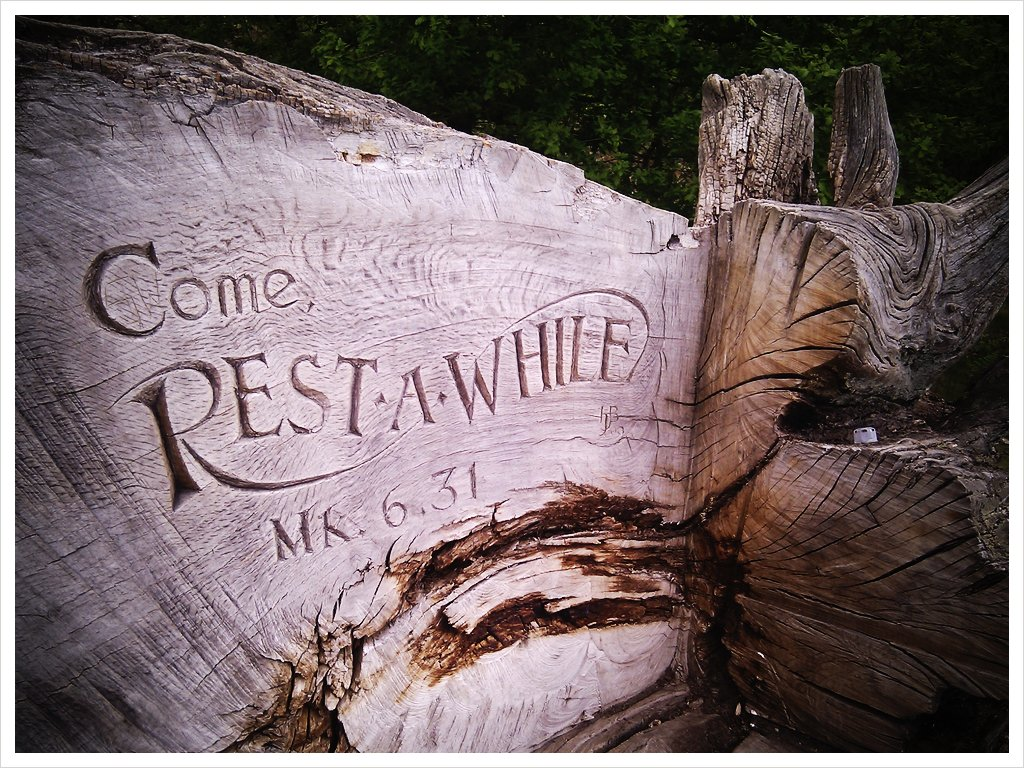
\includegraphics[width=\textwidth]{img/bench}
	        \caption{A bench}
	    \end{subfigure}
	    \caption{Some lights and a bench}
	\end{figure}
\end{frame}


%--------------- slide -------------------
\begin{frame}[fragile]
\frametitle{Caption Style}
\vfill
The \texttt{caption} package has many options for customising the appearance of captions
\vfill
\begin{lstlisting}[style=latexsty]
	\usepackage[font=small, labelfont=bf]{caption}
\end{lstlisting}
\vfill
\end{frame}

%--------------- slide -------------------
\begin{frame}[fragile]
\frametitle{Double Column Floats}
\vfill
When creating a two-column document, it may sometimes be desirable to have your float placed across both columns.
\vfill
This can be done using the \texttt{figure*} and \texttt{table*} environments, which will place tables or images across both columns of a two-column document.
\vfill
Note however, this will force the floats to be either at the top of the page, or on a page of their own.
\vfill
\end{frame}


%--------------- slide -------------------
\begin{frame}[fragile]
\frametitle{Cross Referencing}
\vfill
\vfill
As with tables, our images `float' around the document and so may end up being in a different location to the text describing them. \LaTeX\ provides methods for cross-referencing within documents. 
\vfill
\texttt{{\textbackslash}label} allows us to label floats:
\vfill
\begin{lstlisting}[style=latexsty]
	\label{label_name}
\end{lstlisting}
\vfill
\texttt{{\textbackslash}ref} allows us to refer back to the labelled float or section:
\vfill
\begin{lstlisting}[style=latexsty]
	\ref{label_name}
\end{lstlisting}
\vfill
\texttt{{\textbackslash}pageref} allows us to refer to the page the labelled float or section is on:
\vfill
\begin{lstlisting}[style=latexsty]
	\pageref{label_name}
\end{lstlisting}
\vfill
When using any form of referencing we are required to compile our document twice, so that \LaTeX\ is able to work out where our references should point to within the document.
\vfill
\end{frame}


%--------------- slide -------------------
\begin{frame}[fragile]
\frametitle{Cross Referencing}
\vfill
Labels must be added \emph{after} the caption, but still within the \texttt{figure}, \texttt{subfigure} or \texttt{table} environment.
\vfill
\begin{lstlisting}[style=latexsty]
	Figure~\ref{fig:subfigex} has two subfigures: Figure~\ref{lights} is the image with lights, and Figure~\ref{fig:bench} is the image of a bench.
	\begin{figure}[htbp]
	    \centering
	    \begin{subfigure}{0.3\textwidth}
	        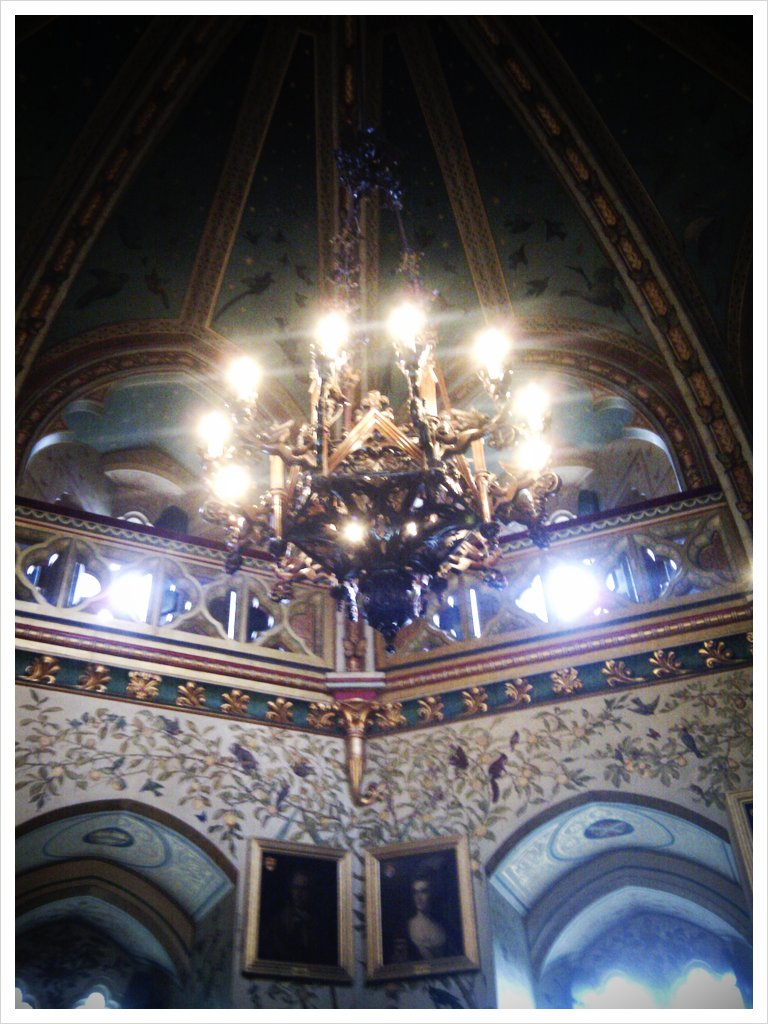
\includegraphics[width=\textwidth]{img/lights}
	        \caption{Some lights} \label{fig:lights}
	    \end{subfigure}
	    \begin{subfigure}{0.3\textwidth}
	        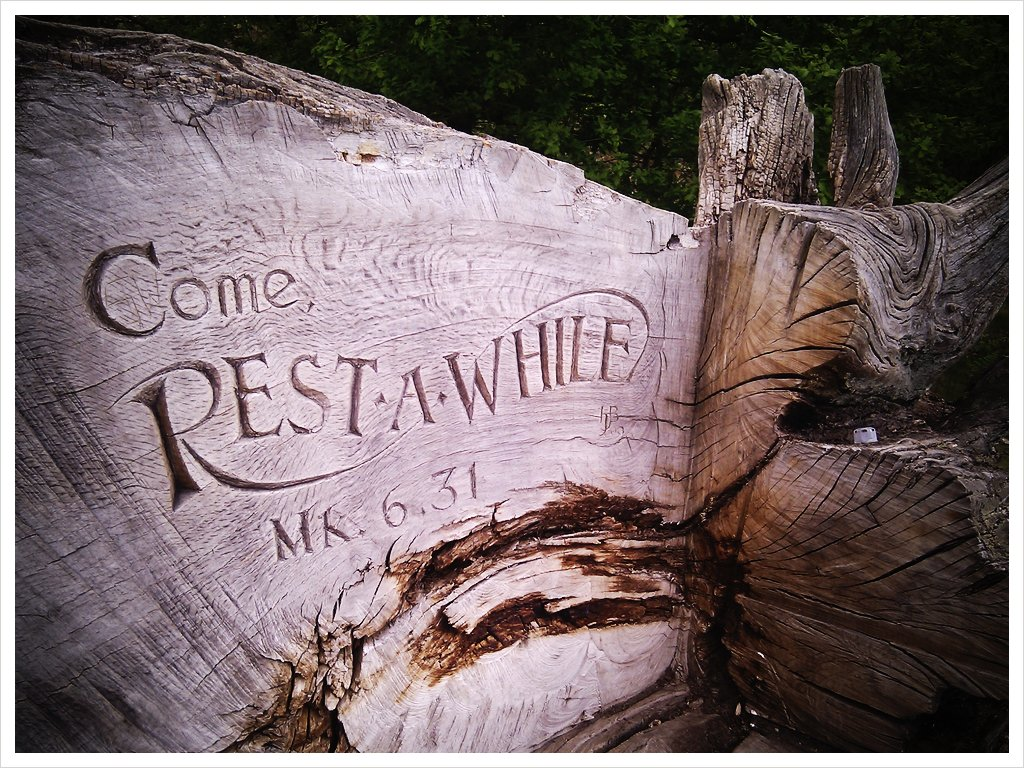
\includegraphics[width=\textwidth]{img/bench}
	        \caption{A bench}  \label{fig:bench}
	    \end{subfigure}
	    \caption{Some lights and a bench} \label{fig:subfigex}
	\end{figure}
\end{lstlisting}
\vfill
\end{frame}

%--------------- slide -------------------
\begin{frame}[fragile]
\frametitle{Cross Referencing}
\vfill
	Figure~\ref{fig:subfigex} has two subfigures: Figure~\ref{fig:lights} is the image with lights, and Figure~\ref{fig:bench} is the image of a bench.
	\begin{figure}[htbp]
	    \centering
	    \begin{subfigure}{0.3\textwidth}
	        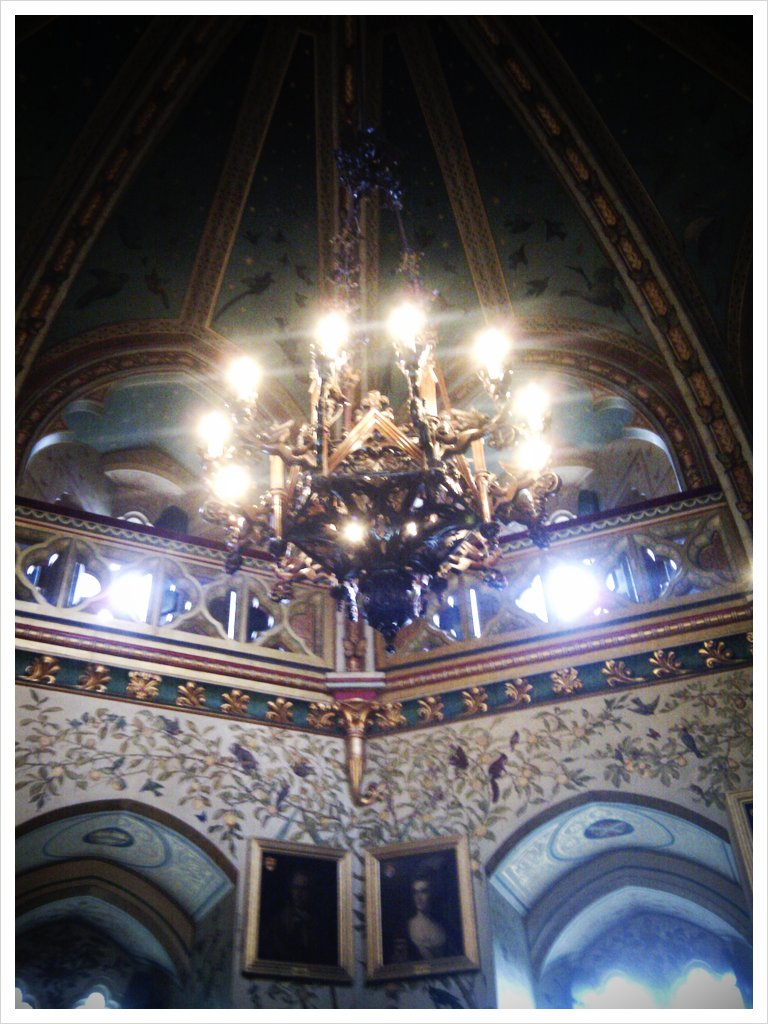
\includegraphics[width=\textwidth]{img/lights}
	        \caption{Some lights} 
	        \label{fig:lights}
	    \end{subfigure}
	    \begin{subfigure}{0.3\textwidth}
	        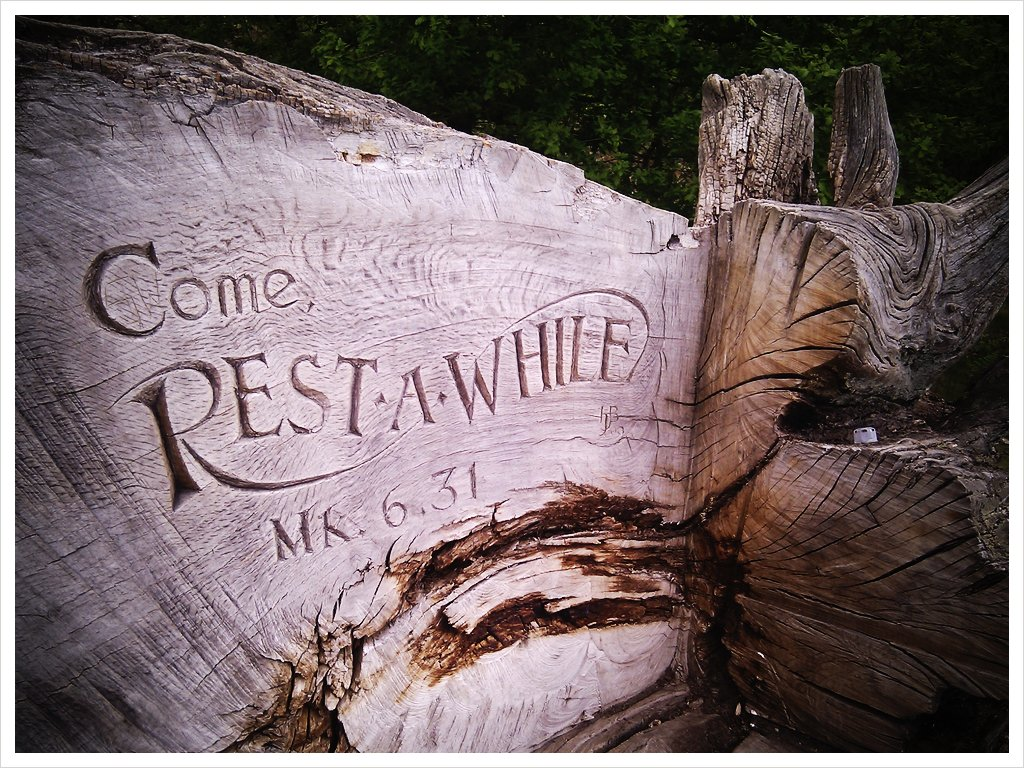
\includegraphics[width=\textwidth]{img/bench}
	        \caption{A bench}  
	        \label{fig:bench}
	    \end{subfigure}
	    \caption{Some lights and a bench} \label{fig:subfigex}
	\end{figure}
\vfill
\end{frame}


%--------------- slide -------------------
\begin{frame}[fragile]
\frametitle{Exercise 2}
\vfill
Experiment with adding images into your documents.
\vfill
Add captions and labels, and refer to them within your text.
\vfill
Experiment with layout and positioning.
\vfill
\end{frame}

%--------------- slide -------------------
\begin{frame}
\frametitle{Help?}
\vfill
There are \emph{many}, \emph{many} places to get more help with \LaTeX. 
\vfill
If you have a problem, use Google! Often that will lead you straight to the documentation for the package or command you have a problem with.
\vfill
Otherwise, StackExchange has a thriving \TeX\ community where you can ask for help and advice: 
\begin{center}
	\texttt{http://tex.stackexchange.com}
\end{center}
\vfill
\end{frame}

%--------------- slide -------------------
\begin{frame}
\frametitle{Help?}
\vfill
All the \LaTeX\ code for the slides and exercises today is available online:
\vfill
\begin{center}
	\texttt{https://github.com/martinjc/LaTeX-an-Introduction--Part-2-}
\end{center}
\vfill
\begin{center}
or
\end{center}
\vfill
\begin{center}
	\texttt{http://martinjc.com}
\end{center}
\end{frame}

\end{document}